\subsection{Front view}
\begin{figure}[h!]
    \centering
    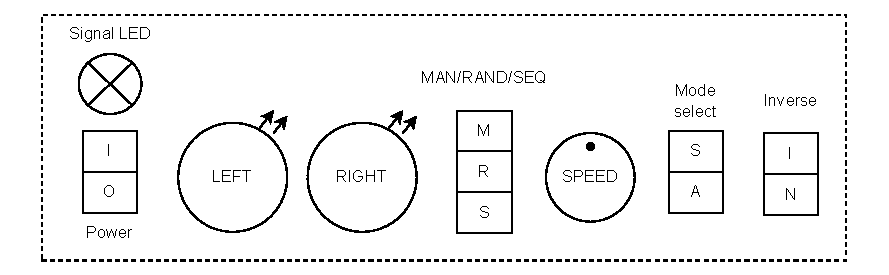
\includegraphics[width=\textwidth]{images/siteshift_frontview.drawio.pdf}
    \caption{Control panel front view.}
    \label{fig:control_panel}
\end{figure}

\subsection{Components}
\begin{description}
    \item[Signal LED] 12 V, 20 mA
    \item[Power switch] A rocker switch rated for at least 2 A
    \item[L/R button] A non-latching push button with 12 V LED backlight.
    \item[State switch] A three-position switch
    \item[Speed potentiometer] 10 k$\Omega$ potentiometer
    \item[Mode/Inverse switch] A two-position switch
\end{description}

\subsection{Wiring}
Each screw terminal for connection is marked with the number 1 on one side; numbering proceeds from that side. An example is shown in figure~\ref{fig:control_panel_wiring}.
\begin{figure}[h!]
    \centering
    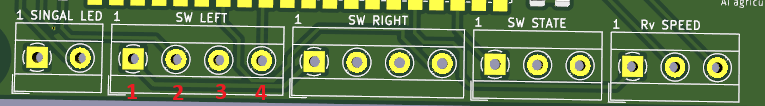
\includegraphics[width=\textwidth]{images/control_panel_wiring.png}
    \caption{Screw terminal numbering.}
    \label{fig:control_panel_wiring}
\end{figure}
\begin{figure}[h!]
    \centering
    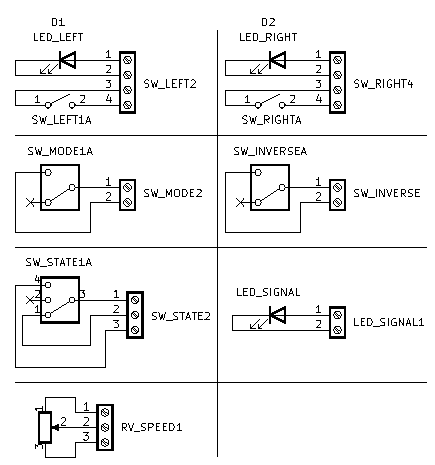
\includegraphics[width=0.8\textwidth]{images/control_panel_schematic.pdf}
    \caption{Control panel connection diagram. Note: This is a connection-only schematic.}
    \label{fig:control_panel_schematic}
\end{figure}

\subsection{Usage}
After turning on the power using the \textbf{power button}, calibration starts automatically. 
Until the calibration is complete, the device cannot be controlled.

The higher a button is placed in this list, the higher its priority.
\begin{description}
    \item[Mode switch] Switches between the state of following the second device synchronous operation (SYN)  
    or the asynchronous state (ASYN), where it is possible to control the device using the    control panel.
    \item[State switch] Three-position switch, allowing switching between manual control, random, and sequential modes.  
    This switch is considered only when ASYN is selected on the previous button.
    \item[L/R buttons] Buttons used to manually move the piston while held.  
    These buttons are active only when the previous switch is set to the manual position.  
    When the buttons are active, the LED backlight is illuminated.
    \item[Speed potentiometer] In asynchronous mode, the potentiometer can be used to set the maximum speed of the piston movement.
\end{description}
The signal LED is active when the device is in any mode other than manual, indicating that the device is active.  
If the device is in synchronous mode and the LED is blinking, this indicates a communication error.
